\pagebreak
\subsection{Implementing Mach Number Jumps}
% [25\%] Implement the mesh adaptation algorithm based on the Mach number jumps. Run your algorithm for $\alpha = 1\degree$ with at least 5 adaptive iterations, and perform the following post-processing: Plot the sequence of your adapted meshes. Plot the Mach number and total pressure fields on your finest mesh. Plot the ATPR output versus number of cells in the mesh -- one data point per adaptive iteration. Discuss the results, including areas targeted for adaption and the convergence of the output.

In this section I will implement an adaptive mesh function that will flag edges shown in Figure \ref{fig:triangle_refinement} given the discrepancy in Mach number across cell edges. The purpose of this function is to refine the mesh in the areas that are more prone to error; most notably the areas where there is large jumps in the Mach number like across shocks. These shocks will be located at the inlet and then trained throughout the interior of the engine. In this section I will refine the mesh and then look at the results of the Mach field, the total pressure, and finally the ATPR at the end of each refinement iteration.

\subsubsection{Adapted Meshes}
In this section, I will implement the Mach jumps into the code to refine the meshes to lower the error in the approximated solution. Using my code I will create a new mesh after each iterative solution and then refine the mesh that will be used on the next approximation. Shown on the following page in Figure \ref{fig:adapted_meshes}, are the meshes after each refinement. Most notable, is that the mesh refines at the location at which oblique shocks are forming -- the interior and inlet of the engine. This refinement makes sense intuitively since shocks provide a discontinuity in the flow which naturally cause large errors in calculation.


\pagebreak
\begin{figure}[h!]
    \centering
    \begin{subfigure}[h]{0.39\linewidth}
        \centering
        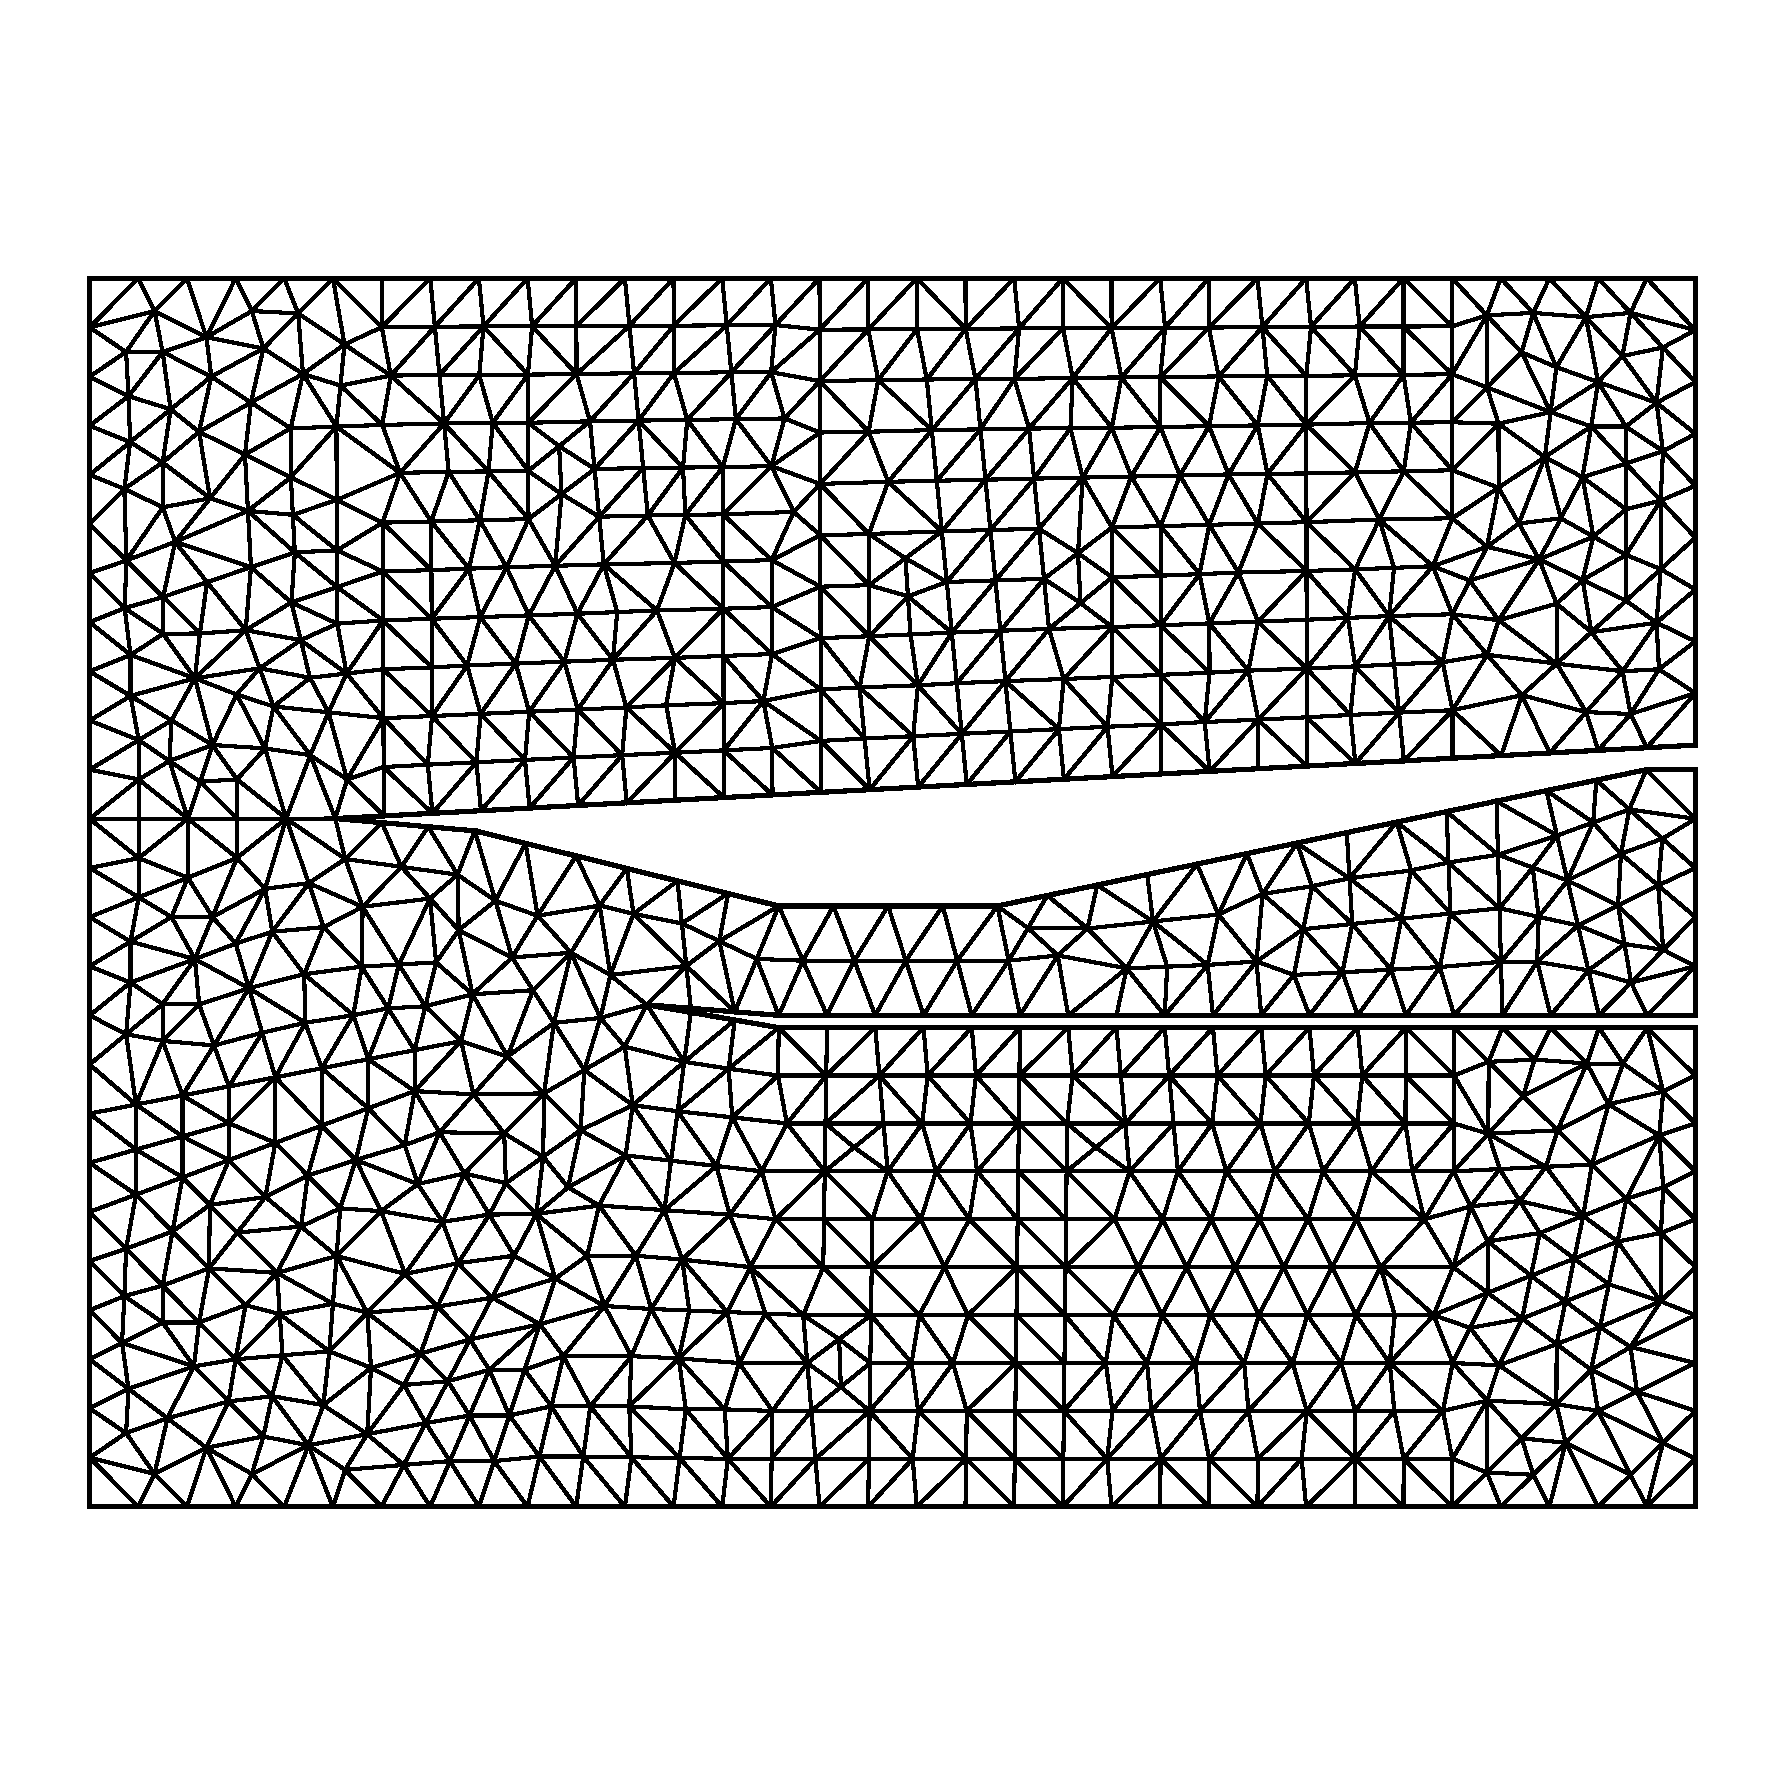
\includegraphics[width=\linewidth]{rep/q4/mesh0.pdf}
        \caption{Baseline mesh.}
    \end{subfigure}
    \begin{subfigure}[h]{0.39\linewidth}
        \centering
        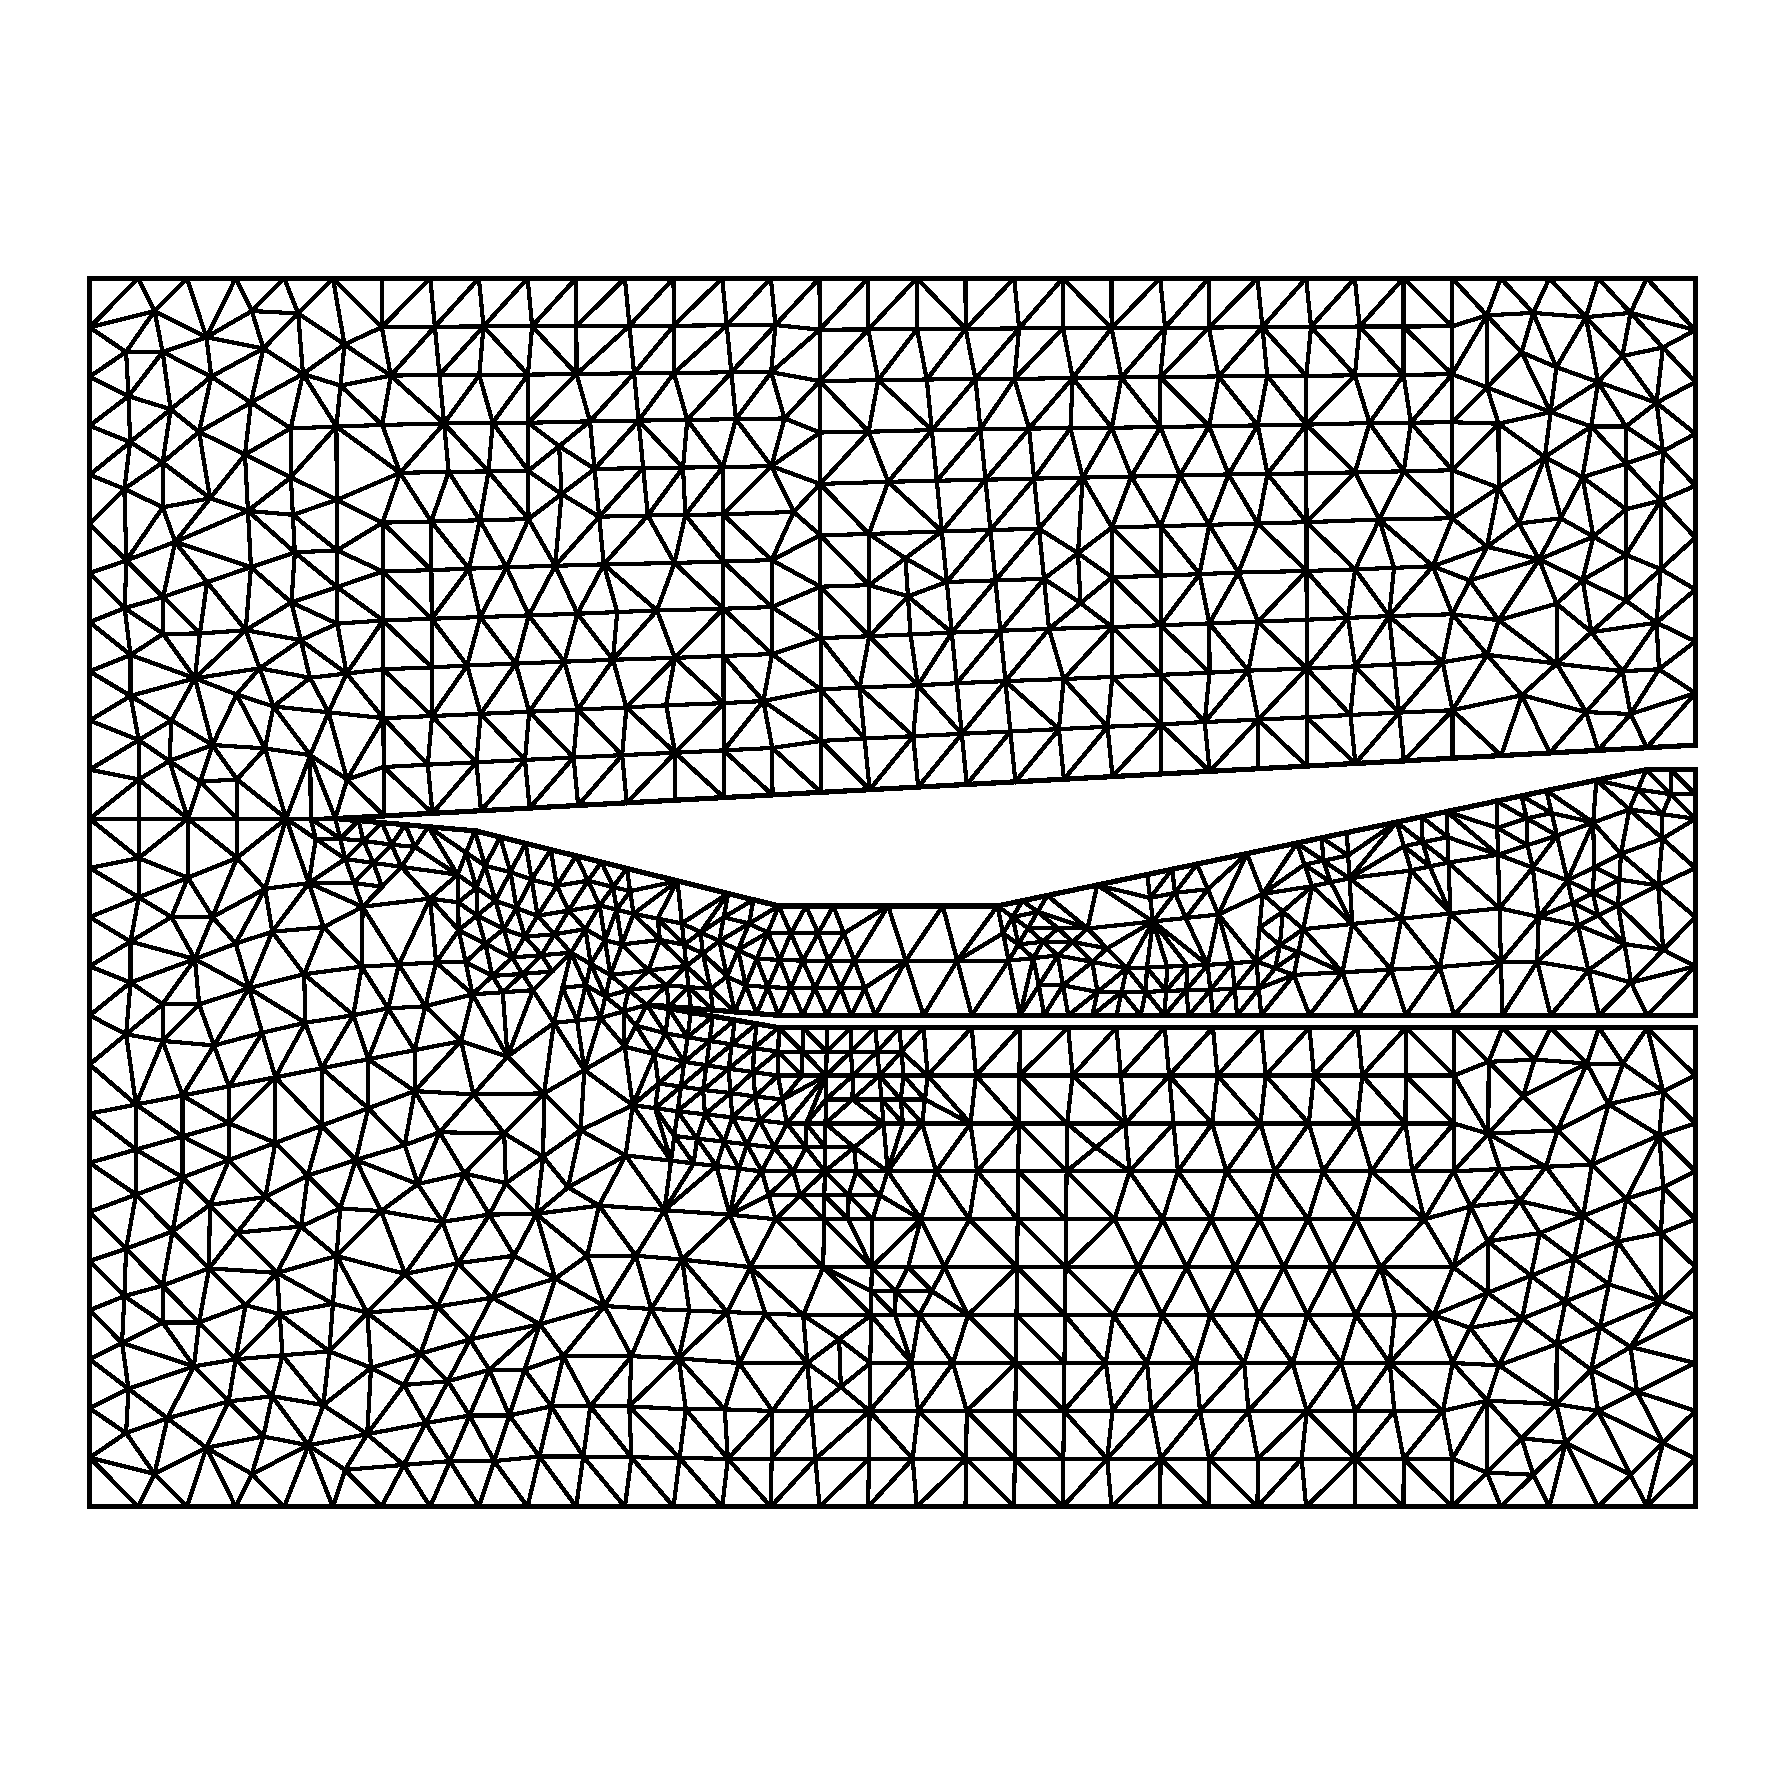
\includegraphics[width=\linewidth]{rep/q4/mesh1.pdf}
        \caption{Adapted mesh, iteration 1.}
    \end{subfigure}

    \begin{subfigure}[h]{0.39\linewidth}
        \centering
        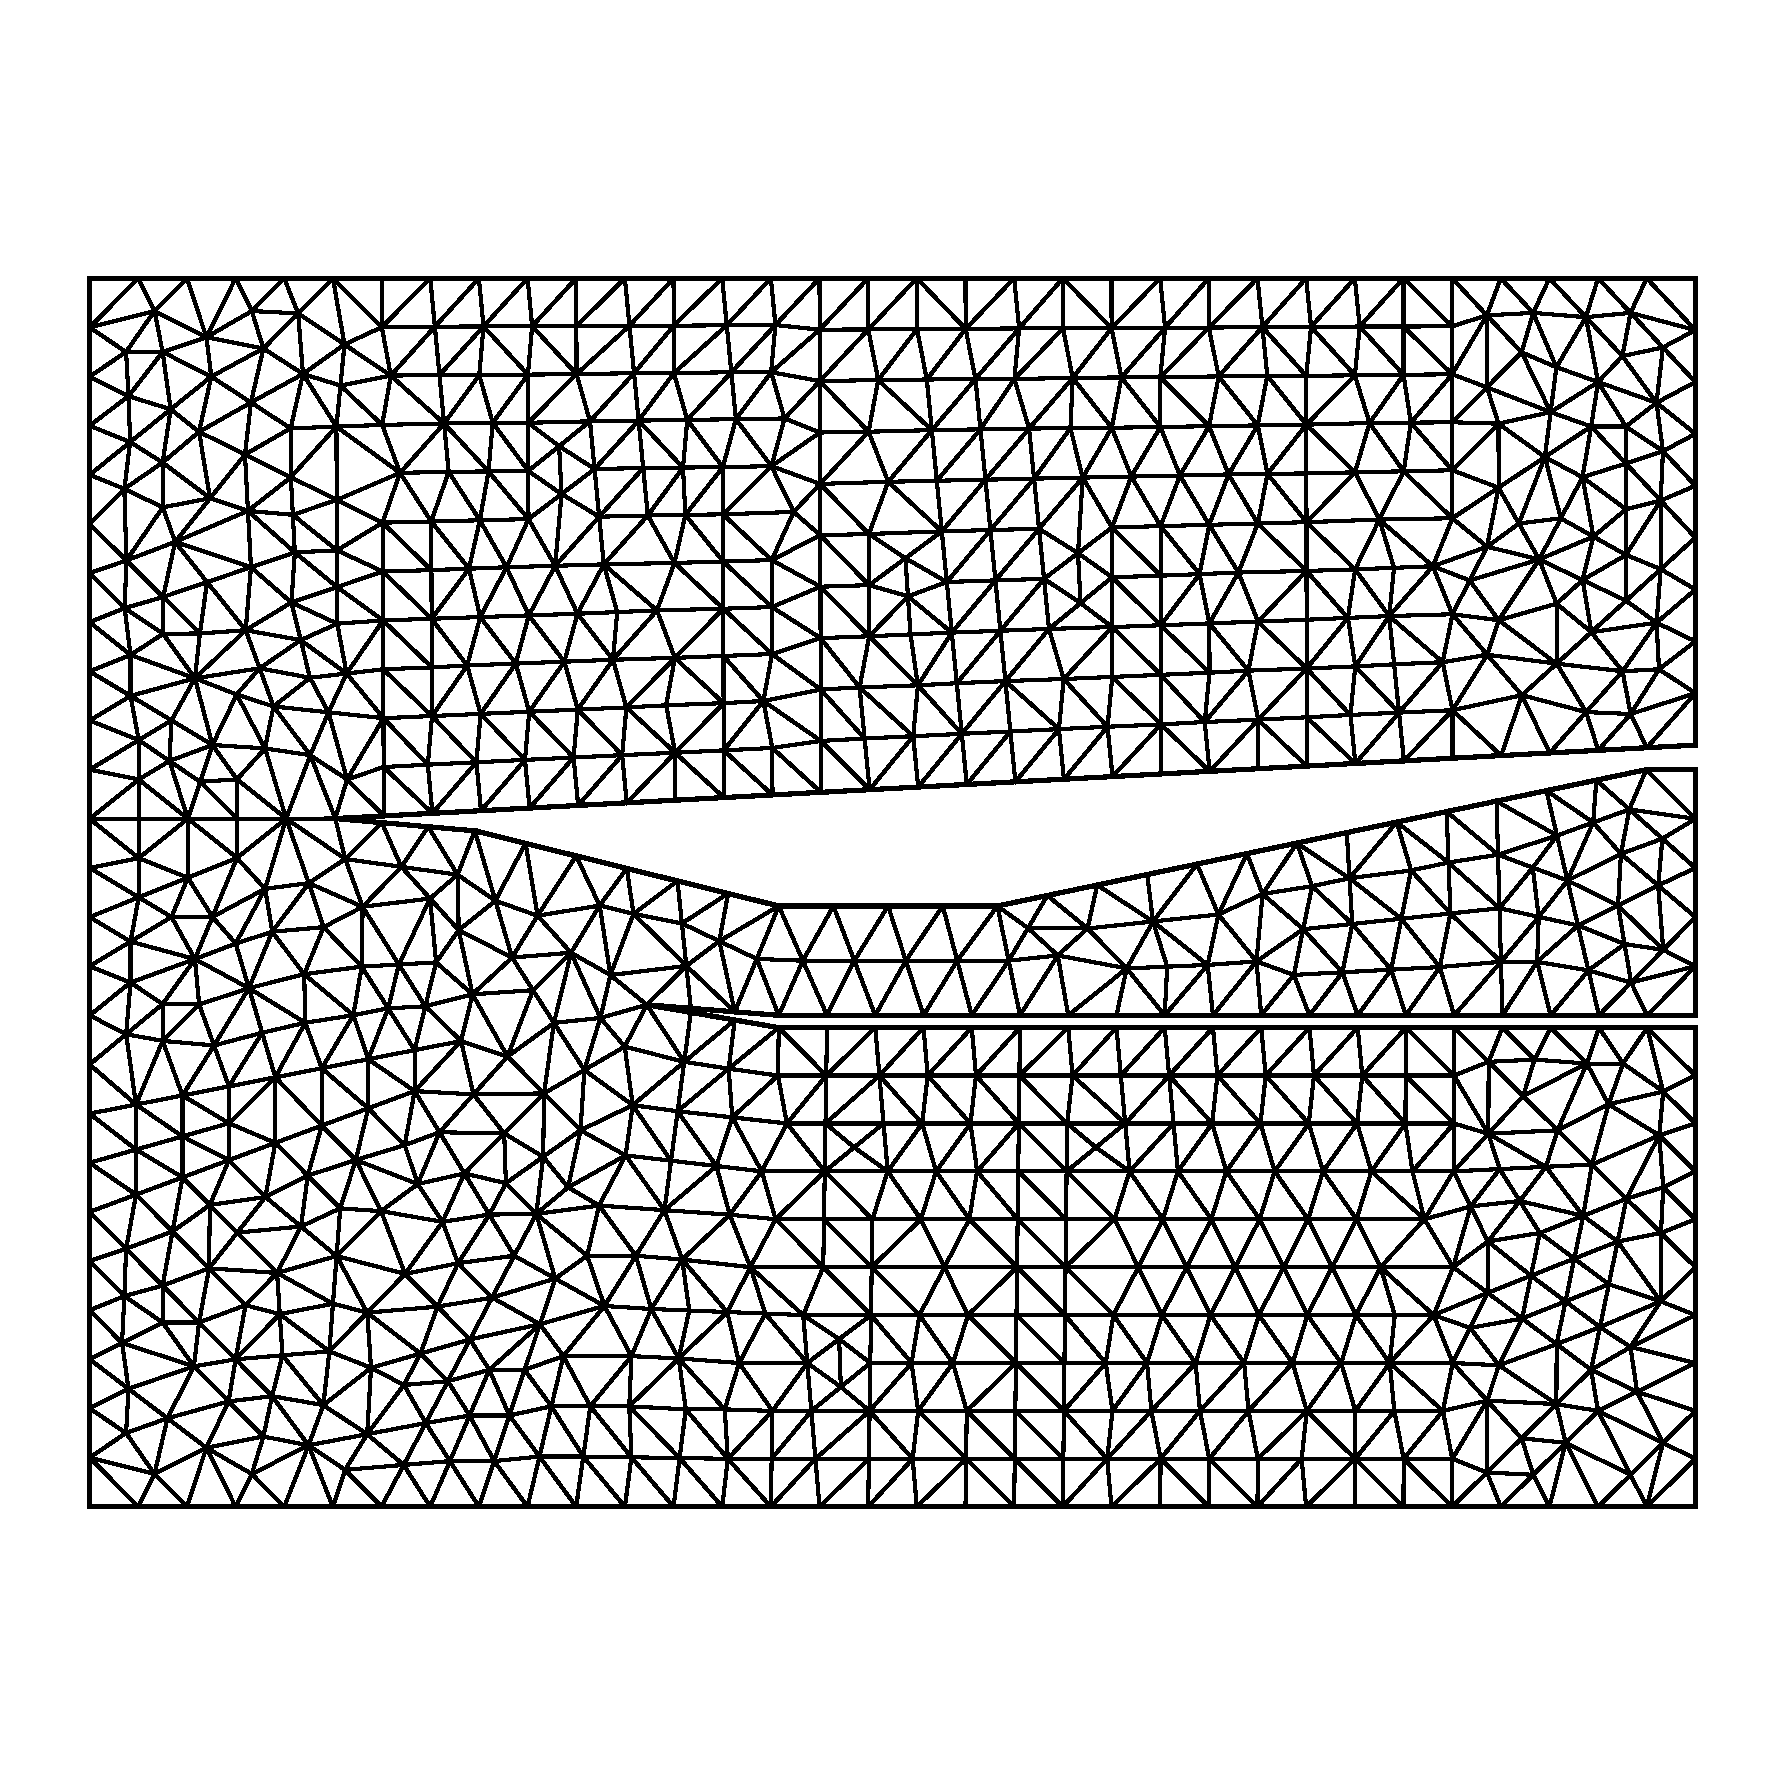
\includegraphics[width=\linewidth]{rep/q4/mesh2.pdf}
        \caption{Adapted mesh, iteration 2.}
    \end{subfigure}
    \begin{subfigure}[h]{0.39\linewidth}
        \centering
        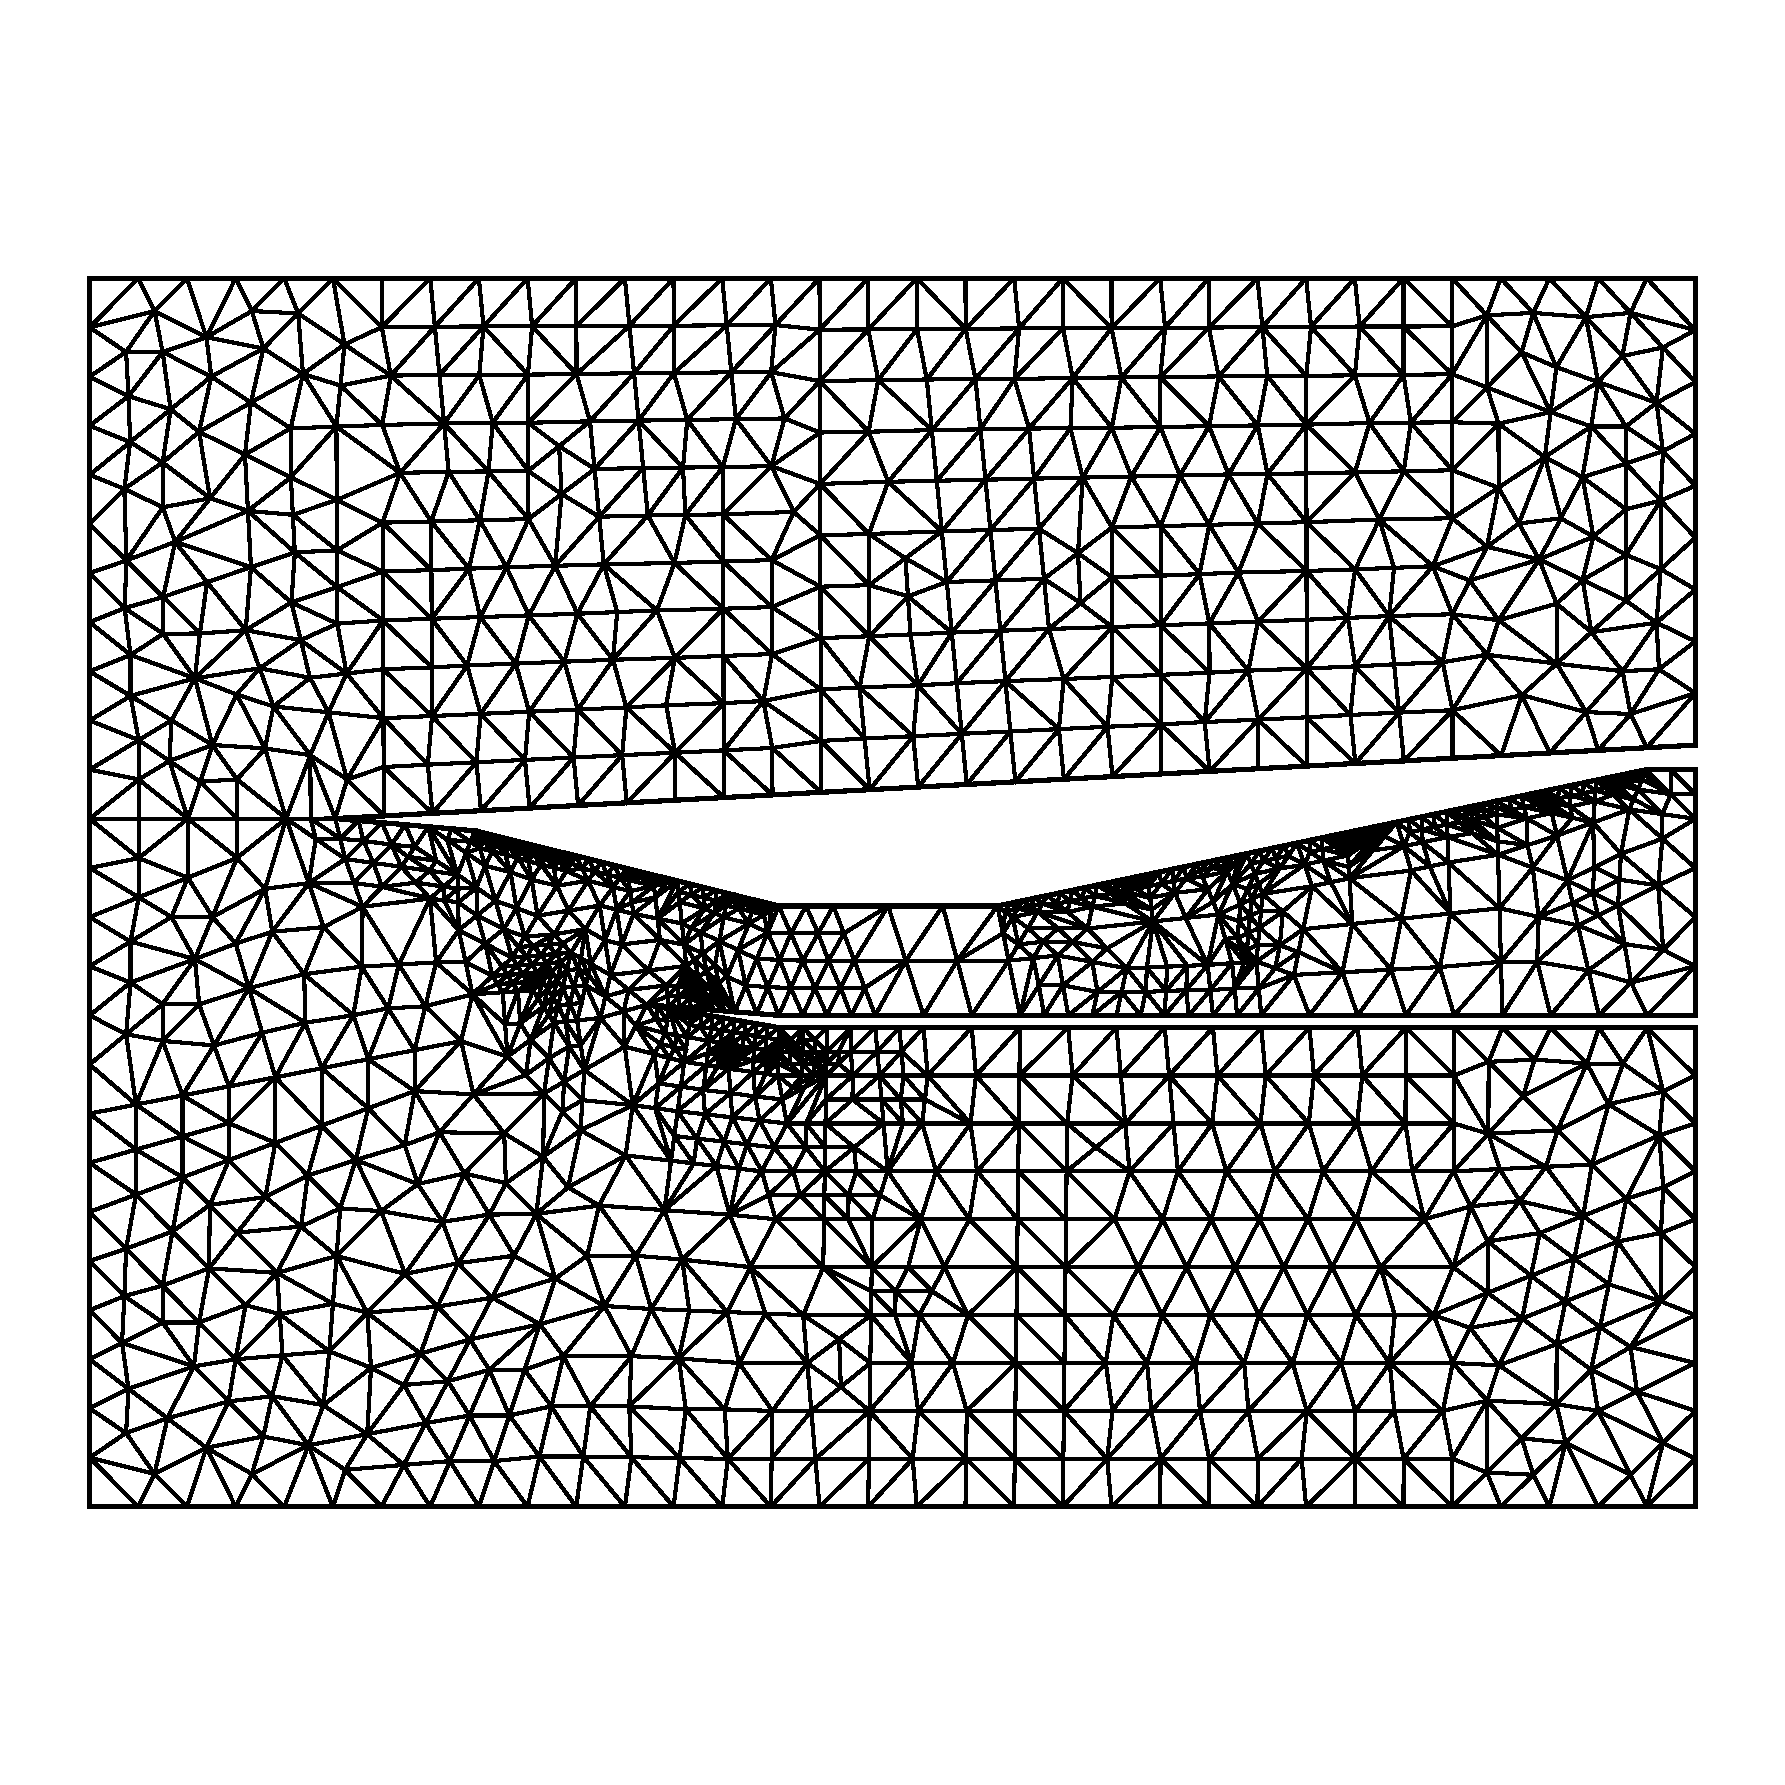
\includegraphics[width=\linewidth]{rep/q4/mesh3.pdf}
        \caption{Adapted mesh, iteration 3.}
    \end{subfigure}

    \begin{subfigure}[h]{0.39\linewidth}
        \centering
        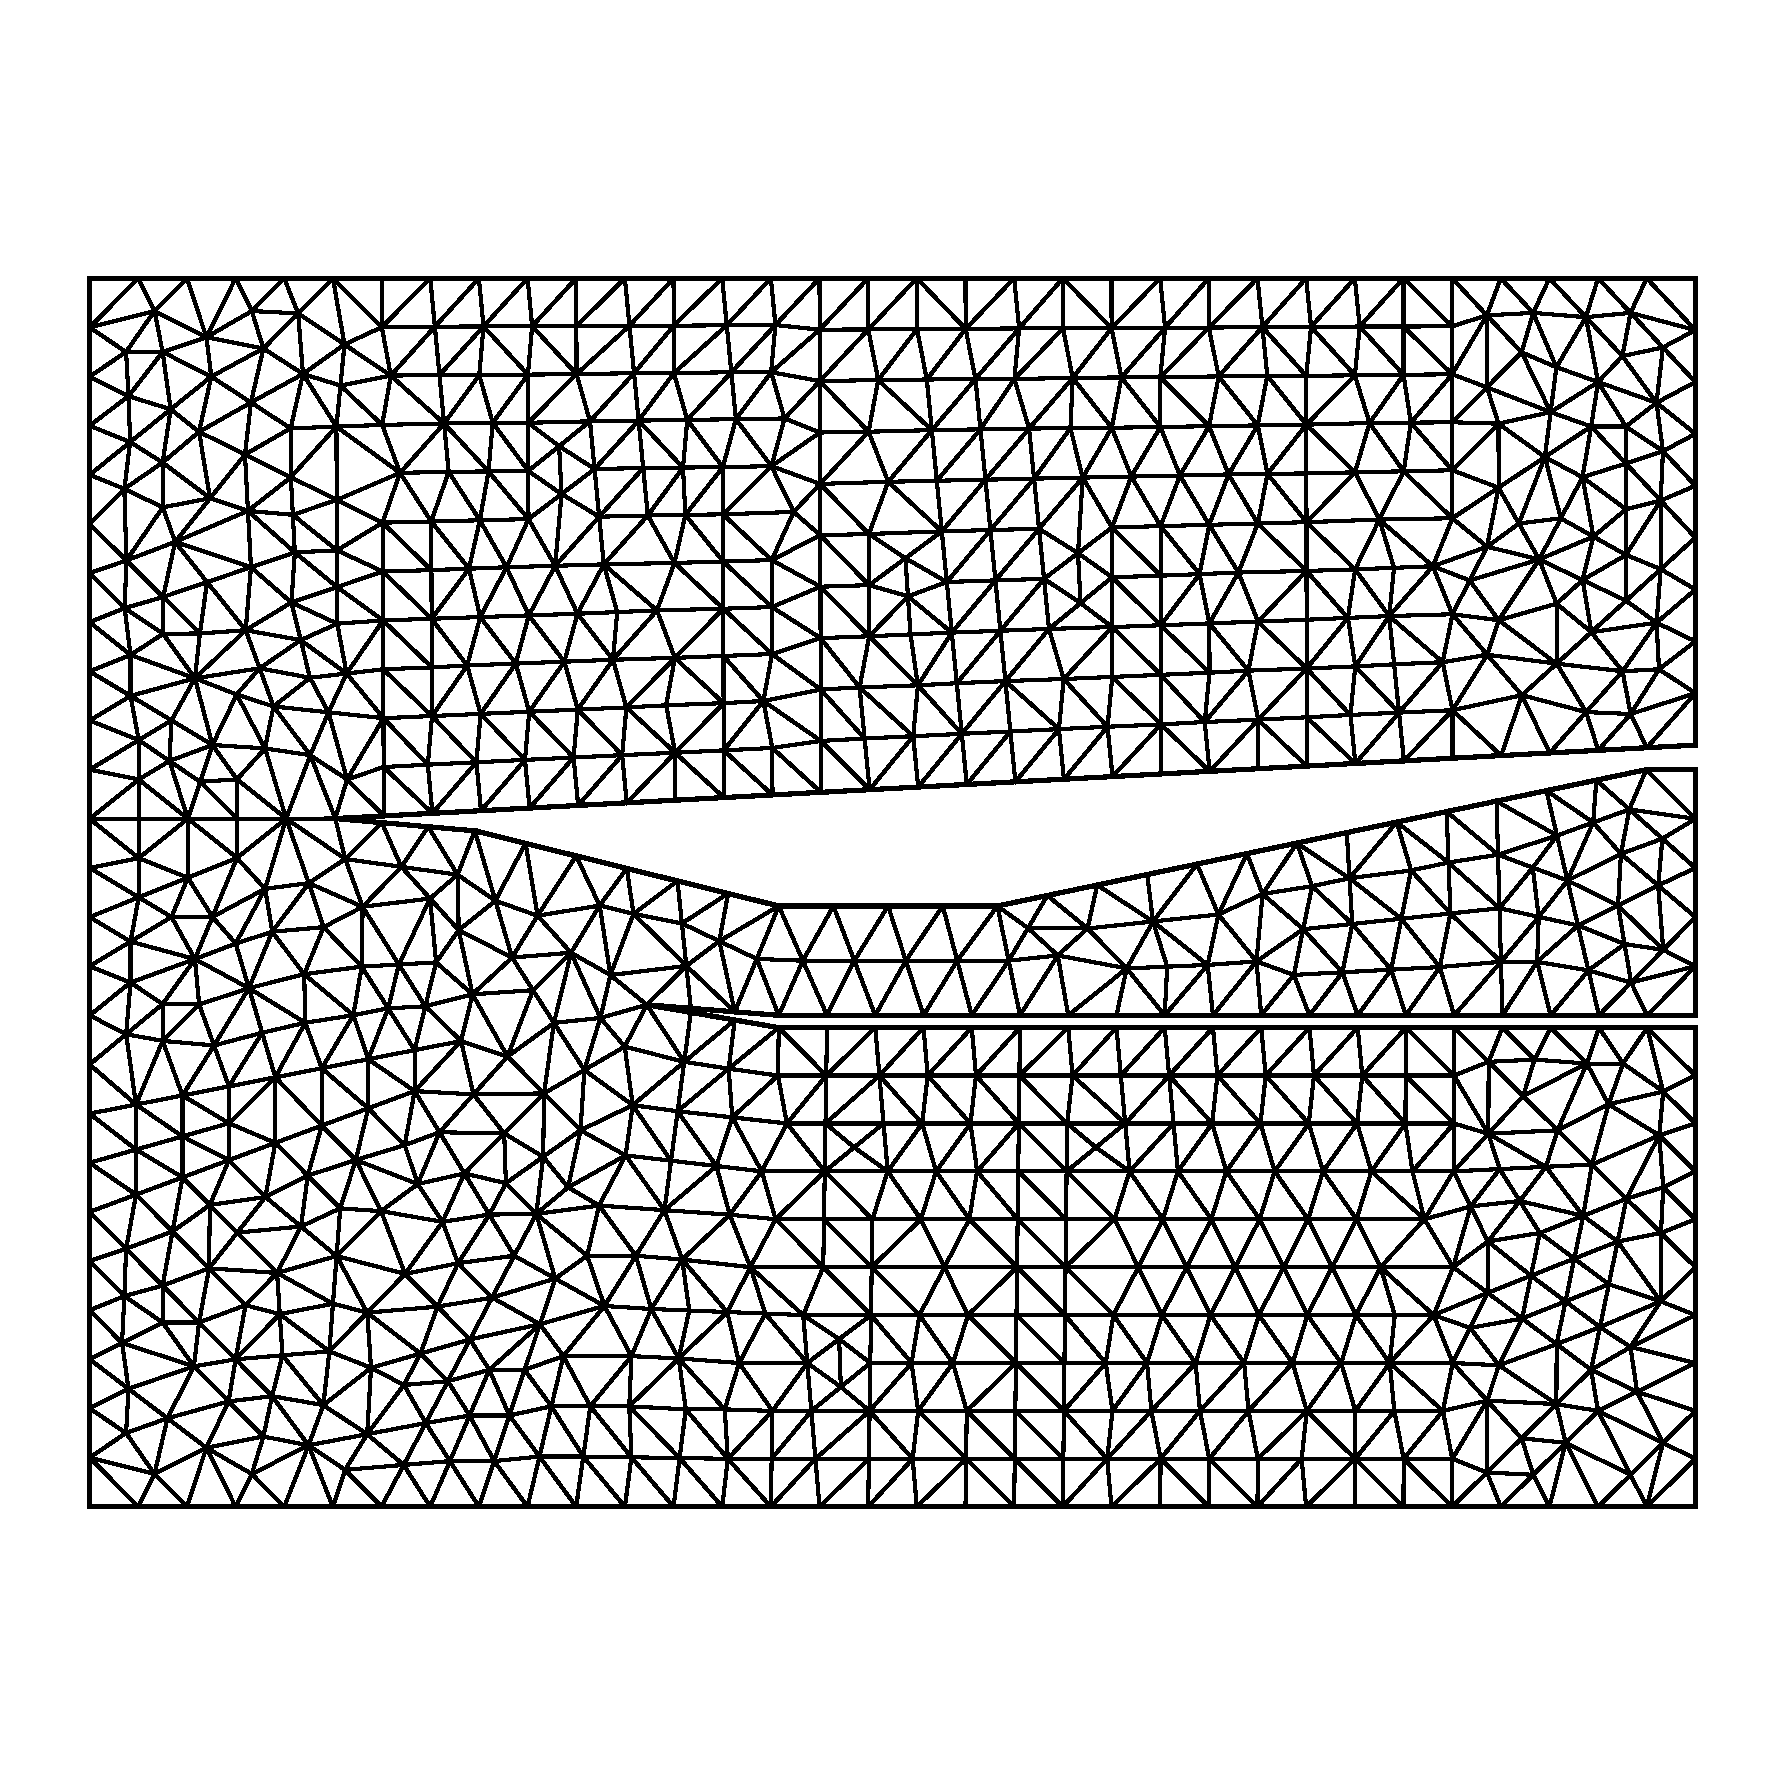
\includegraphics[width=\linewidth]{rep/q4/mesh4.pdf}
        \caption{Adapted mesh, iteration 4.}
    \end{subfigure}
    \begin{subfigure}[h]{0.39\linewidth}
        \centering
        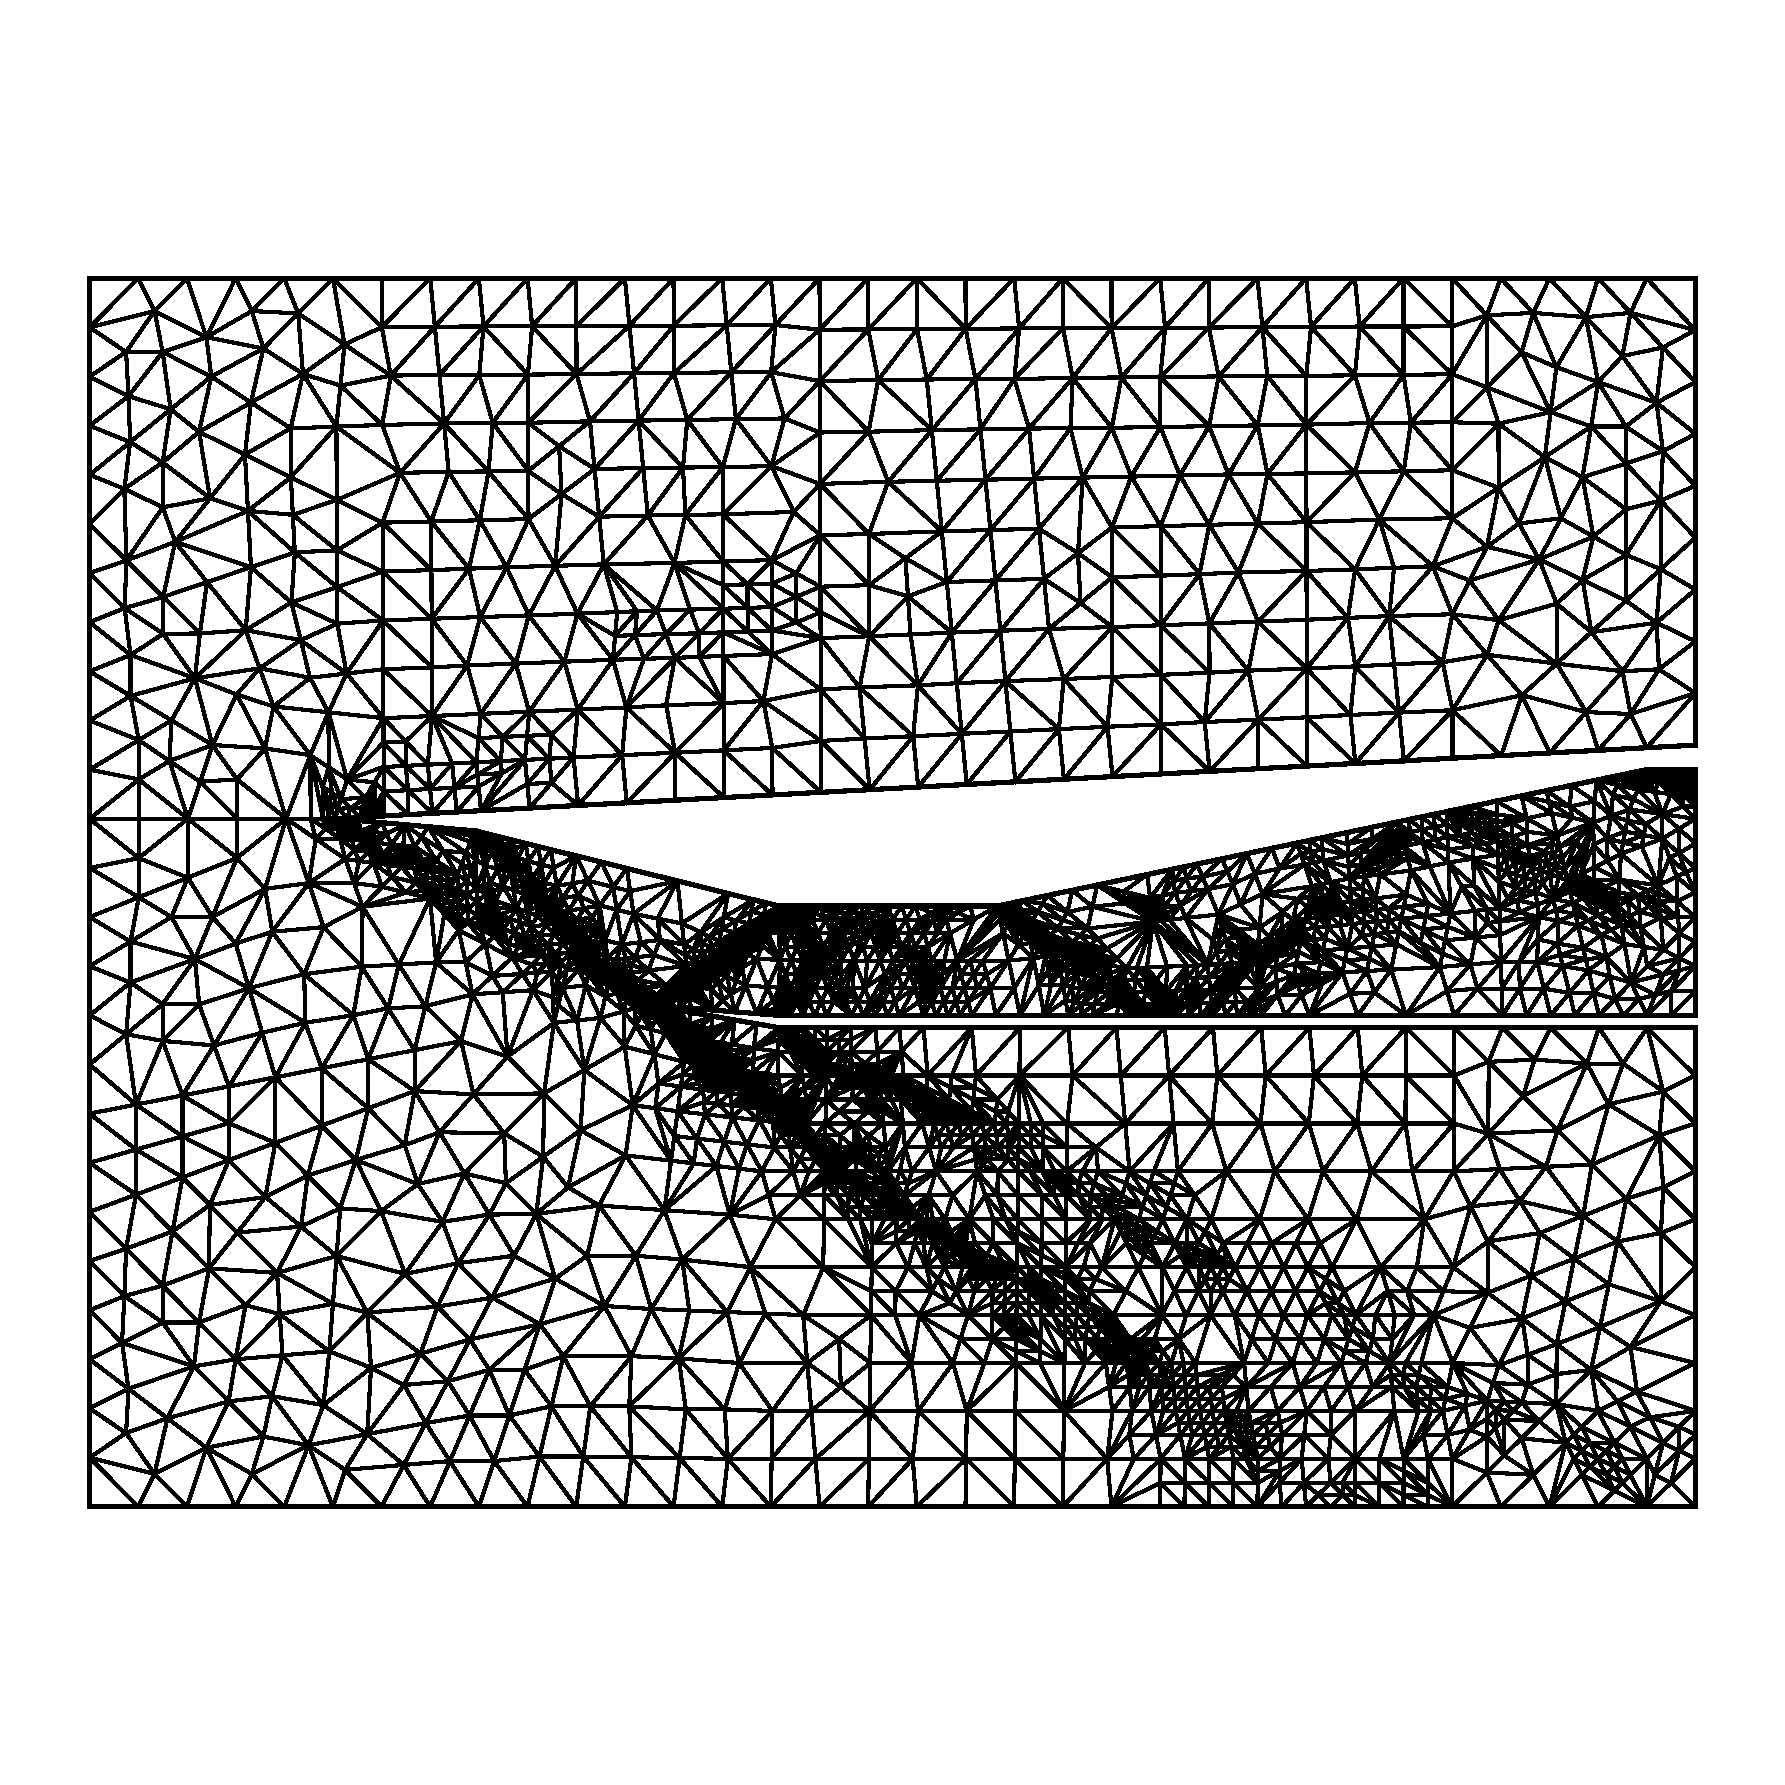
\includegraphics[width=\linewidth]{rep/q4/mesh5.pdf}
        \caption{Adapted mesh, iteration 5.}
    \end{subfigure}
    \caption[Adapted Meshes Versus Baseline Mesh]{Adapted meshes versus baseline mesh.}
    \label{fig:adapted_meshes}
\end{figure}



\pagebreak
\subsubsection{Adapted Mesh Field Plots}
\begin{figure}[h]
    \centering
    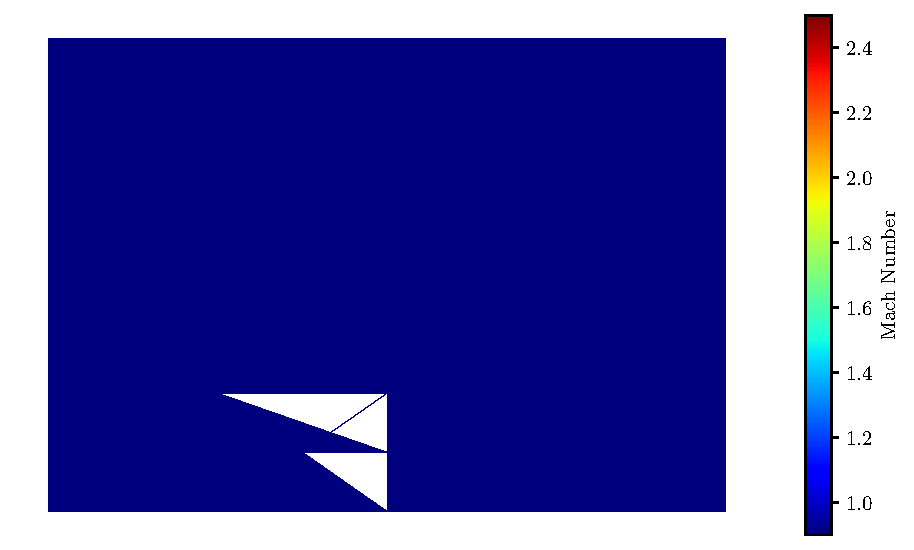
\includegraphics[width = 0.9\linewidth]{rep/q4/Machfield.pdf}
    \caption[Field Plot of Mach Number for Adapted Mesh]{Field plot of Mach number with $\alpha = 1\degree$ for the finest mesh.}
    \label{fig:adapted_mach}
\end{figure}

\paragraph{Finest Mesh Field Plot of Mach Number} Shown above in Figure \ref{fig:adapted_mach}, is the Mach field for the most refined mesh after 5 adaptive iterations. Comparing the results from this refined mesh to that in Figure \ref{fig:mach_mesh0} shows \textcolor{red}{what \ldots}

\pagebreak
\begin{figure}[h]
    \centering
    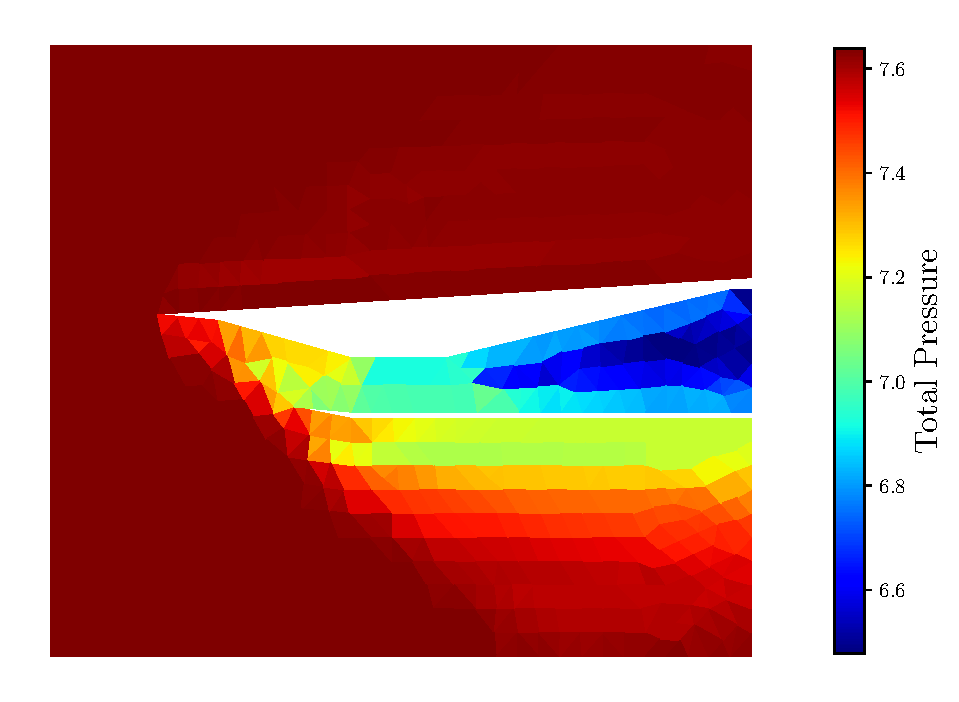
\includegraphics[width = 0.9\linewidth]{rep/q4/Pfield.pdf}
    \caption[Field Plot of Total Pressure for Adapted Mesh]{Field plot of total pressure with $\alpha = 1\degree$ for the finest mesh.}
    \label{fig:adapted_pt}
\end{figure}

\paragraph{Finest Mesh Field Plot of Total Pressure} Shown above in Figure \ref{fig:adapted_pt}, is the total pressure field for the most refined mesh after 5 adaptive iterations. Comparing the results from this refined mesh to that in Figure \ref{fig:pt_mesh0} shows \textcolor{red}{what \ldots}

\pagebreak
\subsubsection{Adapted Mesh ATPR Convergence}
\begin{figure}[h]
    \centering
    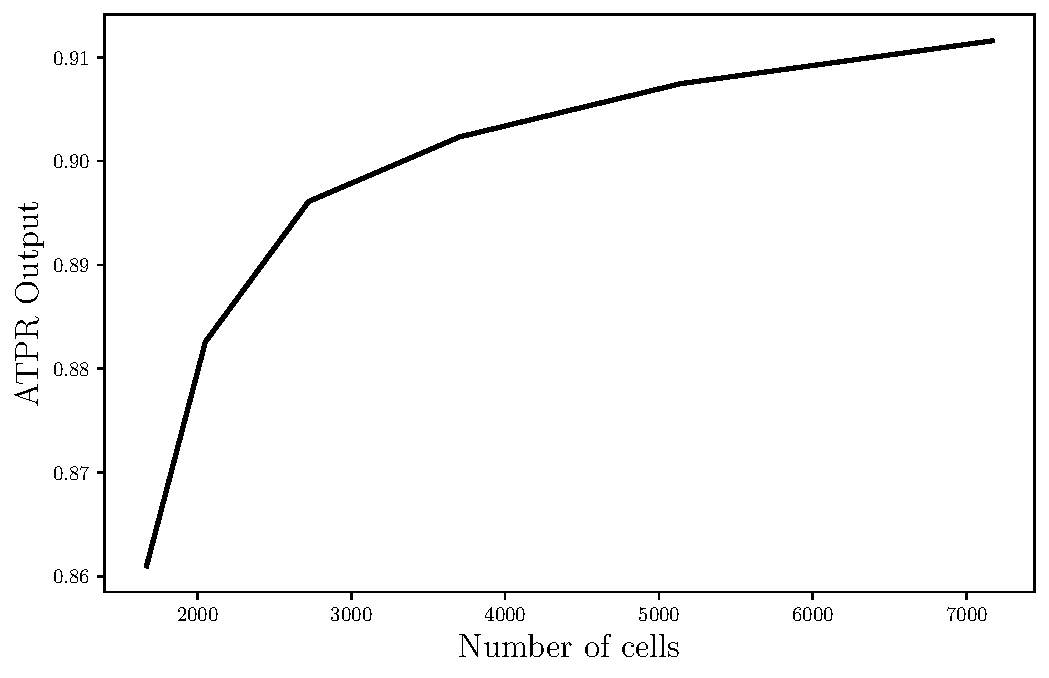
\includegraphics[width = 0.9\linewidth]{rep/q4/ATPR.pdf}
    \caption[ATPR Convergence with Cell Number]{ATPR output versus number of cells in mesh.}
    \label{fig:adapted_ATPR}
\end{figure}

Shown above in Figure \ref{fig:adapted_ATPR}, is the ATPR output versus the number of cells and its effect on the convergence of the ATPR. \textcolor{red}{Discuss \ldots}

